\section{Question 4}
\textit{Décrivez et expliquez les principaux résultats de la référence \cite{tiquette} et comment les auteurs ont résolus le problème du contrôle de zone via l'algorithme de Ford-Fulkerson.}\\~\\\par
L'article donné en référence pour ce projet est à propos d'une étude réalisée par cinq chercheurs aux Etat-Unis. Cette dernière consiste en l'identification de postes de contrôles afin de protéger les grandes villes américaines.\\
Afin de trouver les localisions optimales des points de contrôle, les chercheurs ont trouvés plusieurs approches. Cependant, celle retenue consiste à chercher les points de contrôles minimum permettant de sécuriser la région choisie. Cet ensemble de points de contrôle est le appelé Minimum Cut Set (MCS) en théorie des graphes. En effet, nous pouvons représenter la ville à protéger par un graphe. Les liens seraient alors la représentation des axes de circulation et les nœuds les intersections entre plusieurs axes (un un changement d'état pour un axe). Ainsi, le MCS permet de réaliser une coupe du graphe en deux parties disjointes.\\
Dans notre cas, nous souhaitons avoir le moins de liens à couper afin de ne mettre en place que des points de contrôles stratégiques. Ce problème peut être résolu par l'algorithme de flux maximum de Ford-Fulkerson.\\
Dans le cadre de cette étude, il ne sera pas pris en compte le coût des points de contrôle qui pourront être mis en place.\\
Tout au long de cet articles, les chercheurs se sont focalisés sur les 50 plus grandes villes américaines (c.f. annexe \ref{annexe:1}).\\~\\\par
Dans un premier temps, il est nécessaire de définir deux variables que nous allons réutiliser tout au long de cette explication :
\begin{itemize}
 \item $r_i$, le rayon interne. Celui-ci définie la zone que nous souhaitons protéger. Si un acteur malveillant parvient à rentrer au sein de cette zone, alors nous devons considérer cette dernière comme perdue.
 \item $r_o$, le rayon externe. Celui-ci va correspondre à la zone au sein de laquelle nous allons effectuer nos contrôles.
\end{itemize}
Nous avons ici un système de cercles concentriques. Le cercle interne doit avoir un rayon $r_i$ inférieur ou égal à celui du cercle externe, $r_o$ comme le montre l'image \ref{img:1}. On a ici un rayon interne $r_i$ de $15$ miles ($\approx 24km$) et in rayon externe $r_o$ de $25$ miles ($\approx 40km$).
\begin{figure}[H]
 \centering
 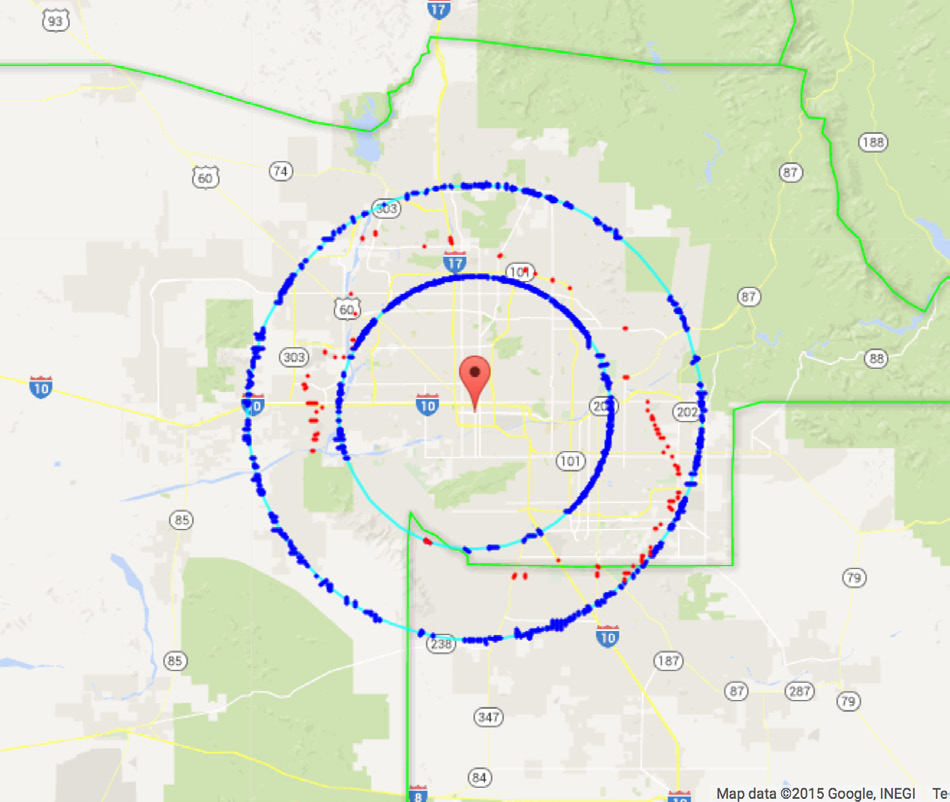
\includegraphics[width=.5\textwidth]{img/circles.png}
 \caption{Représentation des cercles interne et externe pour la ville de Phoenix}
 \label{img:1}
\end{figure}
Ainsi, la zone présente entre les deux cercles peut être qualifiée de \enquote{zone tampon}. C'est au sein de cette dernière que nous allons placer les points de contrôle.\\
Sur l'image \ref{img:1}, nous pouvons retrouver différentes notations :
\begin{itemize}
 \item En bleu clair sont représentés les cercles internes et externes.
 \item En bleu foncé sont représentés les axes et routes s'intersectant avec les cercles.
 \item En rouge sont représentés les routes appartenant à la MCS.
\end{itemize}
Dans notre exemple, nous avons la taille de la MCS, $M(15,25)=64$. Ainsi, nous savons qu'il faudra, en suivant cette configuration 64 points de contrôle afin de pouvoir protéger la zone interne.\\
Si nous prenons un cercle externe plus grand, nous pouvons constater que le nombre de points de contrôle va alors varier :
\begin{figure}[H]
 \centering
 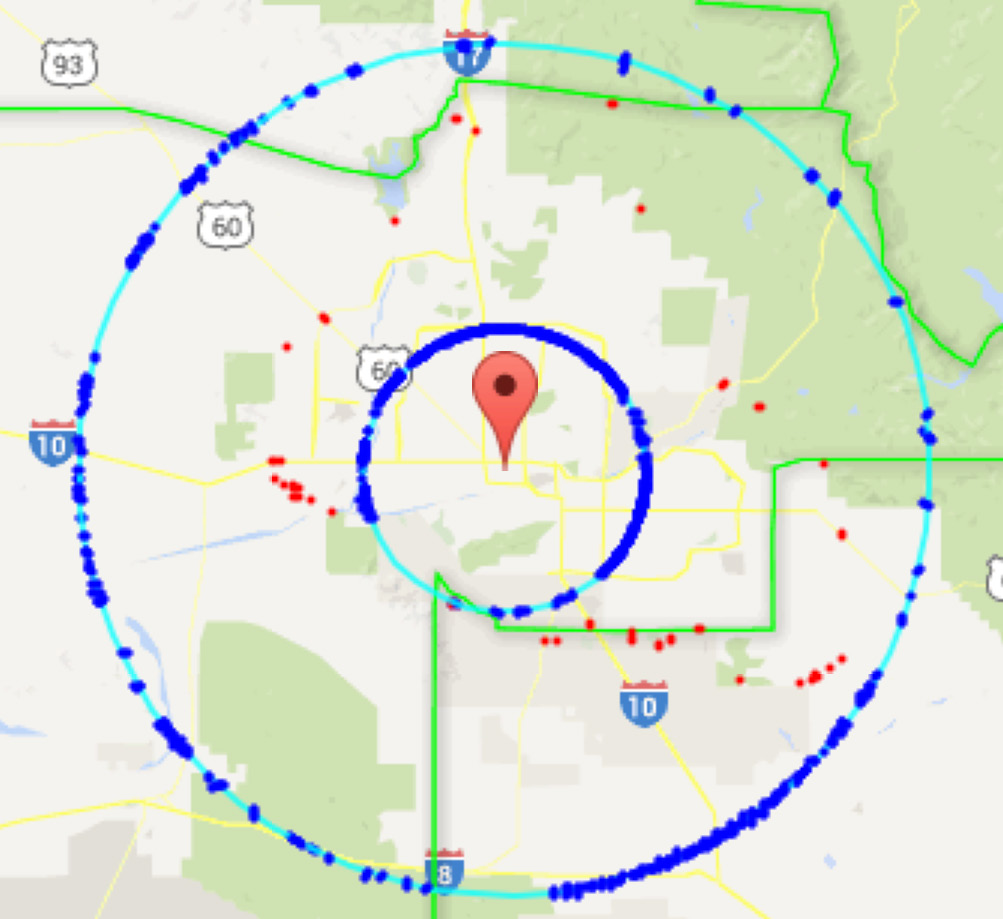
\includegraphics[width=.5\textwidth]{img/circles2.png}
 \caption{Représentation des cercles interne et externe pour la ville de Phoenix avec une MCS $(15,45)$}
 \label{img:2}
\end{figure}
Ici, nous sommes dans une configuration $(15,45)$. Ainsi, nous avons une zone tampon beaucoup plus grande que dans l'exemple précédent. Ainsi, le nombre de points de contrôle va logiquement varier. En effet, en agrandissant la zone tampon, le nombre de routes va changer. Ainsi, nous avons dans notre configuration moins de petits axes coupant notre zone. La proportion de grands axes va alors faire diminuer le nombre de points de contrôles à 36.